\documentclass[preprint,12pt]{elsarticle}

\usepackage{amsmath,amssymb,amsfonts}
\usepackage{graphicx}
\usepackage{textcomp}
\usepackage{xcolor}
\usepackage{booktabs}
\usepackage{multirow}
\usepackage{hyperref}
\usepackage{float}
\usepackage{subcaption}
\usepackage{lineno}
\usepackage{needspace}

% =================================================================================
% FLOAT PLACEMENT -- FIXED (v2)
% v1 used [H] to pin every float exactly at its source location. That
% removed float-pages, but [H] is rigid: if a figure/table does not fit in
% the remaining space on the current page, LaTeX still cannot split it, so
% it pushes the ENTIRE float to a fresh page and leaves whatever room was
% left on the previous page blank -- which is the "short heading, big gap,
% then the figure alone on the next page" pattern seen in v1.
%
% Fix: go back to LaTeX's normal floating ([htbp]) so it has room to slide
% a float a little earlier or later to close the gap, combined with mild
% (not extreme) fraction tuning so a page that is mostly text plus one
% float is still considered acceptable. No \FloatBarrier is used, since
% forcing barriers is what caused floats to pile up into isolated float
% pages in the very first version. \needspace is used once, around the
% short Highlights/Summary Table block, to stop it splitting across pages.
% =================================================================================
\renewcommand{\topfraction}{0.85}
\renewcommand{\bottomfraction}{0.65}
\renewcommand{\textfraction}{0.10}
\renewcommand{\floatpagefraction}{0.70}
\setcounter{topnumber}{3}
\setcounter{bottomnumber}{2}
\setcounter{totalnumber}{4}

% Journal information
\journal{International Journal of Medical Informatics}

\begin{document}

\begin{frontmatter}

% =================================================================================
% TITLE & AUTHORS
% =================================================================================
\title{Cost-Effective Clinical AI for Dementia Progression Forecasting: A Robust Gradient Boosting Framework Using Exclusively Routine Clinical Data from the NACC Cohort}

\author[ruet]{MD Walid Waccub Swadhin}
\ead{waccub@gmail.com}

\cortext[cor1]{Corresponding author}

\affiliation[ruet]{organization={Department of Computer Science and Engineering, Rajshahi University of Engineering and Technology (RUET)},
            city={Rajshahi},
            country={Bangladesh}}

% =================================================================================
% ABSTRACT
% =================================================================================
\begin{abstract}
\textbf{Background and Objective:} Early identification of patients progressing from Mild Cognitive Impairment (MCI) to Alzheimer's Disease (AD) is critical for therapeutic intervention. Current state-of-the-art predictive models predominantly rely on expensive neuroimaging (MRI/PET) or invasive cerebrospinal fluid (CSF) biomarkers, limiting accessibility in primary care and resource-limited settings. This study develops a high-performance, cost-effective, and ethically robust machine learning framework to forecast dementia progression using \textit{exclusively} routine clinical data.

\vspace{0.5em}
\textbf{Methods:} We used longitudinal data from the National Alzheimer's Coordinating Center (NACC) Uniform Data Set, comprising 150,904 clinical visits from 37,633 patients across 40+ Alzheimer's Disease Research Centers. We framed this as a ``Next-Visit Forecasting'' problem, predicting the CDR\textregistered\ Dementia Staging Instrument score (CDR) at time $t+1$ from data at time $t$. We developed a robust XGBoost framework for clinical tabular data, evaluating BorderlineSMOTE and a weighted ensemble as ablations, with patient-level GroupShuffleSplit validation to prevent data leakage and audits for demographic fairness and error severity.

\vspace{0.5em}
\needspace{8\baselineskip}
\textbf{Results:} On an independent test set of 29,939 visits from 7,527 patients, the base XGBoost model achieved \textbf{87.82\%} accuracy, \textbf{85.14\%} macro F1, and \textbf{87.95\%} weighted F1. Class-specific F1-scores were 0.93 (Normal), 0.83 (MCI), 0.77 (Mild), and 0.88 (Severe). Of all misclassifications, 94.9\% were one stage off, with only 0.2\% three stages off. Performance was broadly consistent across sex, age, and race, although limited subgroup sizes for several racial groups preclude definitive fairness conclusions. SHAP analysis identified diagnosis trajectory, current diagnostic state, and age-diagnosis interaction features as the strongest predictors. Adding BorderlineSMOTE or ensembling reduced aggregate performance relative to the base model.

\vspace{0.5em}
\textbf{Conclusions:} Robust dementia risk stratification is achievable using routine clinical assessments, without expensive neuroimaging. A sensitivity analysis excluding all APOE genotype and family-history variables changed macro F1 by only 0.09 percentage points, indicating that the framework does not depend on genetic testing. The framework offers a scalable and transparent tool for clinical decision support in community healthcare and resource-constrained settings, with performance broadly similar across the evaluated demographic subgroups; larger subgroup samples are needed before definitive fairness claims can be made. These results support a ``Frugal AI'' paradigm that democratizes early Alzheimer's detection.
\end{abstract}

\begin{keyword}
Alzheimer's Disease \sep Clinical Forecasting \sep Ensemble Learning \sep NACC Dataset \sep Algorithmic Fairness \sep Explainable AI \sep Dementia Progression \sep Machine Learning in Healthcare
\end{keyword}

\end{frontmatter}

\begin{samepage}
\section*{Highlights}
\begin{itemize}
    \item Routine clinical data forecast next-visit dementia status.
    \item Patient-level splitting prevents longitudinal data leakage.
    \item Base XGBoost achieves 87.82\% accuracy and 85.14\% macro F1.
    \item A roadmap links model outputs to primary-care EHR workflows.
\end{itemize}

\section*{Summary Table}
\begin{itemize}
    \item A clinical-only XGBoost model predicts four next-visit dementia stages.
    \item Evaluation used 29,939 visits from 7,527 previously separated patients.
    \item The study defines prospective validation and EHR translation steps.
\end{itemize}
\end{samepage}

\linenumbers

% =================================================================================
% 1. INTRODUCTION
% =================================================================================
\section{Introduction}

Alzheimer's disease (AD) is a progressive neurodegenerative disorder and the leading cause of dementia, affecting over 55 million people worldwide~\cite{alz2024,gbd2019}. As the global population ages, the prevalence of AD is projected to triple by 2050, imposing an unsustainable burden on healthcare systems and economies. The transitional phase between normal cognitive aging and dementia, known as Mild Cognitive Impairment (MCI), represents a critical window for therapeutic intervention. Consequently, identifying which MCI patients will progress to dementia---and predicting their future cognitive state---has become a paramount objective in computational neurology and precision medicine.

\subsection{The Accessibility Gap in Current AI Models}

Recent advances in Artificial Intelligence (AI) and machine learning have yielded models capable of predicting AD progression with remarkable accuracy; throughout this work, ``progression'' refers specifically to the next recorded CDR-based dementia stage rather than to the underlying neuropathological process. However, many studies rely on multimodal data, including MRI, PET, or cerebrospinal fluid biomarkers. These approaches are costly or invasive, require specialist facilities concentrated in academic centers, and often use smaller datasets that increase overfitting risk; consequently, they are difficult to generalize and scale to population screening.

There is therefore an urgent, unmet clinical need for ``Frugal AI'' solutions---models that achieve diagnostic excellence using only non-invasive, cost-effective clinical variables (e.g., demographics, cognitive assessments, medical history, functional status) that can be routinely collected during standard clinical encounters.

\subsection{Methodological Challenges: Imbalance and Fairness}

Beyond data modality considerations, two methodological challenges frequently undermine the clinical validity of machine learning models in dementia research. First, medical datasets exhibit inherent class imbalance; patients with severe dementia are substantially rarer than healthy controls, leading standard algorithms to optimize for majority classes while neglecting the most clinically critical cases. Our dataset demonstrates a 4.7:1 imbalance ratio between the most and least prevalent classes.

Second, algorithmic fairness has emerged as a critical concern in healthcare AI~\cite{obermeyer2019,rajkomar2018,gianfrancesco2018}. Models trained on demographically skewed populations (predominantly white, highly educated, urban-dwelling participants) may fail to generalize equitably to diverse demographic groups, potentially exacerbating existing healthcare disparities. This concern is particularly acute in dementia research, where socioeconomic factors influence both disease presentation and healthcare access.

\subsection{Contributions and Novelty}

To address these gaps, this study presents a comprehensive framework for robust prediction of the next-visit CDR-based dementia stage using \textit{exclusively} NACC clinical data. Our key contributions are:

\begin{itemize}
    \item \textbf{Clinical-Only Next-Visit Forecasting:} We demonstrate state-of-the-art performance using an optimized Gradient Boosting Machine (XGBoost), proving that expensive neuroimaging is not strictly necessary for accurate risk stratification. Unlike static cross-sectional classification, our model explicitly predicts the \textit{future} CDR-based diagnostic stage ($t+1$), providing actionable prognostic information. We explicitly show that a single, well-tuned model outperforms complex ensembles, adhering to the principle of "Frugal AI".

    \item \textbf{Rigorous Validation with Leakage Prevention:} We implement patient-level GroupShuffleSplit validation, ensuring no patient's data appears in both training and test sets---a common methodological flaw in longitudinal studies that artificially inflates performance metrics.

    \item \textbf{Comprehensive Fairness Audit:} We conduct systematic performance evaluation across Age, Sex, and Race subgroups, quantifying disparities and ensuring the model is equitable for diverse populations.

    \item \textbf{Clinically-Meaningful Error Analysis:} Beyond aggregate accuracy, we analyze the \textit{severity} of misclassifications (1-stage vs. 2-stage vs. 3-stage errors), demonstrating that even when the model errs, predictions remain clinically proximal to ground truth.

    \item \textbf{Interpretable Feature Attribution:} We employ SHAP (SHapley Additive exPlanations) values to provide transparent, clinician-interpretable explanations of model predictions, aligning with regulatory requirements for explainable AI in healthcare.
\end{itemize}

Several recent studies have addressed closely related prediction tasks. Prior work has applied survival and clinical-variable models to the NACC and ADNI cohorts to predict progression~\cite{pang2023,song2023,arnold2025}, and deep recurrent architectures have been applied to multimodal longitudinal data for next-visit prediction~\cite{alolaimat2023}; machine learning on NACC has also been applied to related clinical outcomes~\cite{yew2024}. The closest published precedent is a recent XGBoost model trained on NACC and externally validated on a Latvian clinical cohort~\cite{kannenieks2026}. Our contribution differs in three respects: we predict a four-class, patient-level next-visit CDR-based stage rather than a binary or three-class conversion outcome; we use a deliberately simple clinical-tabular model rather than multimodal recurrent networks; and we add explicit demographic-fairness and error-severity audits.

% =================================================================================
% 2. MATERIALS AND METHODS
% =================================================================================
\section{Materials and Methods}

\subsection{Dataset and Study Population}

Data were obtained from the National Alzheimer's Coordinating Center (NACC) Uniform Data Set (UDS)~\cite{nacc2022}. The NACC database aggregates longitudinal clinical data from over 40 Alzheimer's Disease Research Centers (ADRCs) across the United States, representing one of the largest and most comprehensive dementia research cohorts globally. Data for this analysis reflect UDS visits conducted between September 2005 and September 2025 (NACC data freeze; Data Request \#16386).

\textbf{Inclusion Criteria:} We selected participants who had at least two consecutive clinical visits to facilitate longitudinal prediction (enabling $t \rightarrow t+1$ forecasting). \textbf{Exclusion Criteria:} Visits with missing target labels (Clinical Dementia Rating) were excluded.

The final dataset comprised \textbf{150,904 clinical visits} from \textbf{37,633 unique patients}, with an average of 4.0 visits per patient (range: 1--19 visits). Table~\ref{tab:demographics} presents the demographic characteristics of the study population stratified by current diagnostic status.

\begin{table}[H]
\caption{Baseline Characteristics of Study Population by Diagnostic Group}
\label{tab:demographics}
\begin{center}
\footnotesize
\resizebox{\textwidth}{!}{%
\begin{tabular}{lccccc}
\toprule
\textbf{Variable} & \textbf{Total} & \textbf{Normal} & \textbf{MCI} & \textbf{Mild} & \textbf{Severe} \\
\midrule
N (samples) & 150,904 & 79,333 (52.6\%) & 43,594 (28.9\%) & 16,466 (10.9\%) & 11,511 (7.6\%) \\
Age (years) & 74.3$\pm$10.0 & 73.6$\pm$10.0 & 75.0$\pm$9.5 & 74.8$\pm$10.4 & 75.8$\pm$10.8 \\
Female & 88,309 (58.5\%) & 52,230 (65.8\%) & 21,789 (50.0\%) & 7,880 (47.9\%) & 6,410 (55.7\%) \\
Education (yrs) & 16.0$\pm$6.1 & 16.4$\pm$5.7 & 15.9$\pm$5.7 & 15.5$\pm$7.5 & 15.2$\pm$7.8 \\
Race: White & 124,728 (82.7\%) & 64,642 (81.5\%) & 36,068 (82.7\%) & 14,242 (86.5\%) & 9,776 (84.9\%) \\
\bottomrule
\end{tabular}%
}
\end{center}
\end{table}

\subsection{Feature Engineering}

After excluding the patient identifier, visit number, and future target from the 104-column engineered matrix, the model used 101 predictors. Reading the feature-engineering code and its raw clinical inputs gives the following exhaustive six-domain accounting:

\begin{enumerate}
    \item \textbf{Demographics and visit context (16 features):} Eight raw demographic/context variables (age, sex, education, race, ethnicity, marital status, residence, and handedness), seven age-derived variables (baseline age, years in study, age$^2$, three age-risk indicators, and the age--diagnosis product), and visit number.

    \item \textbf{Diagnosis trajectory (17 features):} The current diagnosis, four one-hot current-diagnosis indicators, three lagged diagnoses, first-visit and stability/progression indicators, progression speed, diagnosis-change count, stability score, diagnosis mean and standard deviation, and worst diagnosis ever recorded. Historical diagnosis features were computed from prior visits for each patient; the current diagnosis is retained as a predictor of the subsequent target.

    \item \textbf{Genetic risk (10 features):} Five raw APOE/family-history variables and five engineered APOE4 indicators and age-risk features. APOE genotype is included here as one of the routine clinical/family-history variables used by the framework; its practical availability varies by care setting.

    \item \textbf{Comorbidity and medical history (37 features):} Twenty-eight raw cardiovascular, neurological, metabolic, functional, behavioral, and medication variables, plus nine engineered cardiovascular, neurological, metabolic, and total-burden indicators.

    \item \textbf{Physiologic and temporal features (18 features):} Eight raw anthropometric, vital-sign, and sensory variables plus ten visit-to-visit change and rolling-mean features for BMI, blood pressure, heart rate, and weight.

    \item \textbf{Interaction features (3 features):} Age $\times$ APOE4, age $\times$ cardiovascular burden, and education $\times$ current diagnosis.
\end{enumerate}

\subsection{Target Variable Definition}

The prediction target was the Global Clinical Dementia Rating (CDRGLOB) at the \textit{subsequent} visit ($t+1$). We mapped CDR scores into four diagnostic classes:
\begin{itemize}
    \item \textbf{Class 0 (Normal):} CDR = 0
    \item \textbf{Class 1 (MCI):} CDR = 0.5 (Questionable impairment)
    \item \textbf{Class 2 (Mild Dementia):} CDR = 1.0
    \item \textbf{Class 3 (Severe Dementia):} CDR $\geq$ 2.0 (Moderate to Severe)
\end{itemize}

The target distribution exhibited class imbalance: Normal 50.8\%, MCI 26.5\%, Mild 10.8\%, Severe 11.9\%, yielding a 4.7:1 imbalance ratio.

\subsection{Data Preprocessing}

Missing values in numerical features (e.g., BMI, blood pressure) were imputed using median values stratified by current diagnosis class to preserve biological variance. Categorical variables were label-encoded. Infinite values were clipped to prevent numerical overflow.

\textbf{Patient-Level Data Splitting:} To prevent data leakage---a critical flaw where a patient's longitudinal visits appear in both training and test sets, artificially inflating accuracy~\cite{kapoor2023}---we employed \texttt{GroupShuffleSplit} stratification. All visits belonging to a specific patient ID (\texttt{NACCID}) were assigned exclusively to either the Training set (80\%, 120,965 visits from 30,106 patients) or Test set (20\%, 29,939 visits from 7,527 patients). Zero patient overlap was verified between partitions. This study is reported in accordance with the TRIPOD+AI guidance for clinical prediction models that use machine learning~\cite{collins2024,collins2021}.

\subsection{Gradient Boosting Framework}

We implemented a predictive framework based on \textbf{XGBoost} \cite{chen2016}, selected for its performance on tabular clinical data and ability to handle missing values natively. The base XGBoost model without oversampling was the final model used for all downstream analyses.

\textbf{Primary Model Configuration:}
\begin{itemize}
    \item \textbf{Algorithm:} XGBoost Classifier
    \item \textbf{Objective:} Multi-class Softmax
    \item \textbf{Key Hyperparameters:} 1000 estimators, learning rate 0.01, max depth 12, histogram tree method.
    \item \textbf{Regularization:} L1 ($\alpha=0.3$) and L2 ($\lambda=1.0$) regularization were applied to prevent overfitting on the high-dimensional clinical feature space.
\end{itemize}

\textbf{Comparative Ensemble:}
To evaluate the necessity of additional complexity, we also evaluated a weighted ensemble comprising XGBoost, LightGBM \cite{ke2017}, and CatBoost \cite{prokhorenkova2018} as an ablation configuration. The ensemble prediction $P_{\text{ens}}$ was computed as:
\begin{equation}
    P_{\text{ens}}(y|x) = 0.35 \cdot P_{\text{XGB}}(y|x) + 0.35 \cdot P_{\text{LGB}}(y|x) + 0.30 \cdot P_{\text{Cat}}(y|x)
\end{equation}

All models utilized early stopping (100 rounds) with 20\% validation holdout from training data.

\subsection{Class Imbalance Handling}

We evaluated \textbf{BorderlineSMOTE} \cite{han2005}---a variant of the Synthetic Minority Over-sampling Technique (SMOTE) \cite{chawla2002}---only in the designated ablation configurations. When used, it was applied exclusively to the training subset after GroupShuffleSplit partitioning, ensuring that the test set contained only real, unaugmented patient visits. The final Config 1 model used no SMOTE.

Class weights were computed using inverse frequency weighting with empirical multipliers optimized for minority class performance: Normal=0.49, MCI=1.42, Mild=6.93, Severe=5.23.

\subsection{Fairness and Explainability Analysis}

To ensure equitable model performance, we evaluated accuracy and F1-macro scores stratified by:
\begin{itemize}
    \item \textbf{Sex:} Male vs. Female
    \item \textbf{Age Groups:} $<$65, 65--74, 75--84, 85+ years
    \item \textbf{Race:} White, Black/African American, Asian, American Indian/Alaska Native, Native Hawaiian/Pacific Islander, Other/Multiracial, and Unknown (code 99)
\end{itemize}

For interpretability, we applied SHAP \cite{lundberg2017} TreeExplainer to identify feature contributions to predictions across all diagnostic classes.

% =================================================================================
% 3. RESULTS
% =================================================================================
\section{Results}

\subsection{Overall Classification Performance}

The proposed framework was evaluated on the independent test set of 29,939 visits from 7,527 unique patients. Table~\ref{tab:results} summarizes performance metrics for the optimal model configuration.

\begin{table}[htbp]
\caption{Classification Performance on Independent Test Set}
\label{tab:results}
\begin{center}
\begin{tabular}{lcccc}
\toprule
\textbf{Diagnosis Class} & \textbf{Precision} & \textbf{Recall} & \textbf{F1-Score} & \textbf{Support} \\
\midrule
Normal (CDR 0)      & 0.95 & 0.92 & 0.93 & 15,080 \\
MCI (CDR 0.5)       & 0.80 & 0.85 & 0.83 & 8,044 \\
Mild (CDR 1.0)      & 0.74 & 0.80 & 0.77 & 3,257 \\
Severe (CDR $\geq$2) & 0.93 & 0.83 & 0.88 & 3,558 \\
\midrule
\textbf{Macro Average} & \textbf{0.85} & \textbf{0.85} & \textbf{0.85} & 29,939 \\
\midrule
\multicolumn{4}{l}{\textbf{Overall Accuracy}} & \textbf{0.8782} \\
\multicolumn{4}{l}{\textbf{Macro F1-Score}} & \textbf{0.8514} \\
\multicolumn{4}{l}{\textbf{Weighted F1-Score}} & \textbf{0.8795} \\
\bottomrule
\end{tabular}
\end{center}
\end{table}

The base XGBoost model achieved an overall accuracy of \textbf{87.82\%}, a macro F1-score of \textbf{85.14\%}, and a weighted F1-score of \textbf{87.95\%}. The normalized confusion matrix (Figure~\ref{fig:cm_norm}) shows recall of 92.0\% for Normal, 85.0\% for MCI, 80.0\% for Mild, and 83.0\% for Severe cases, with most errors occurring between adjacent diagnostic stages.

\begin{figure}[htbp]
\centering
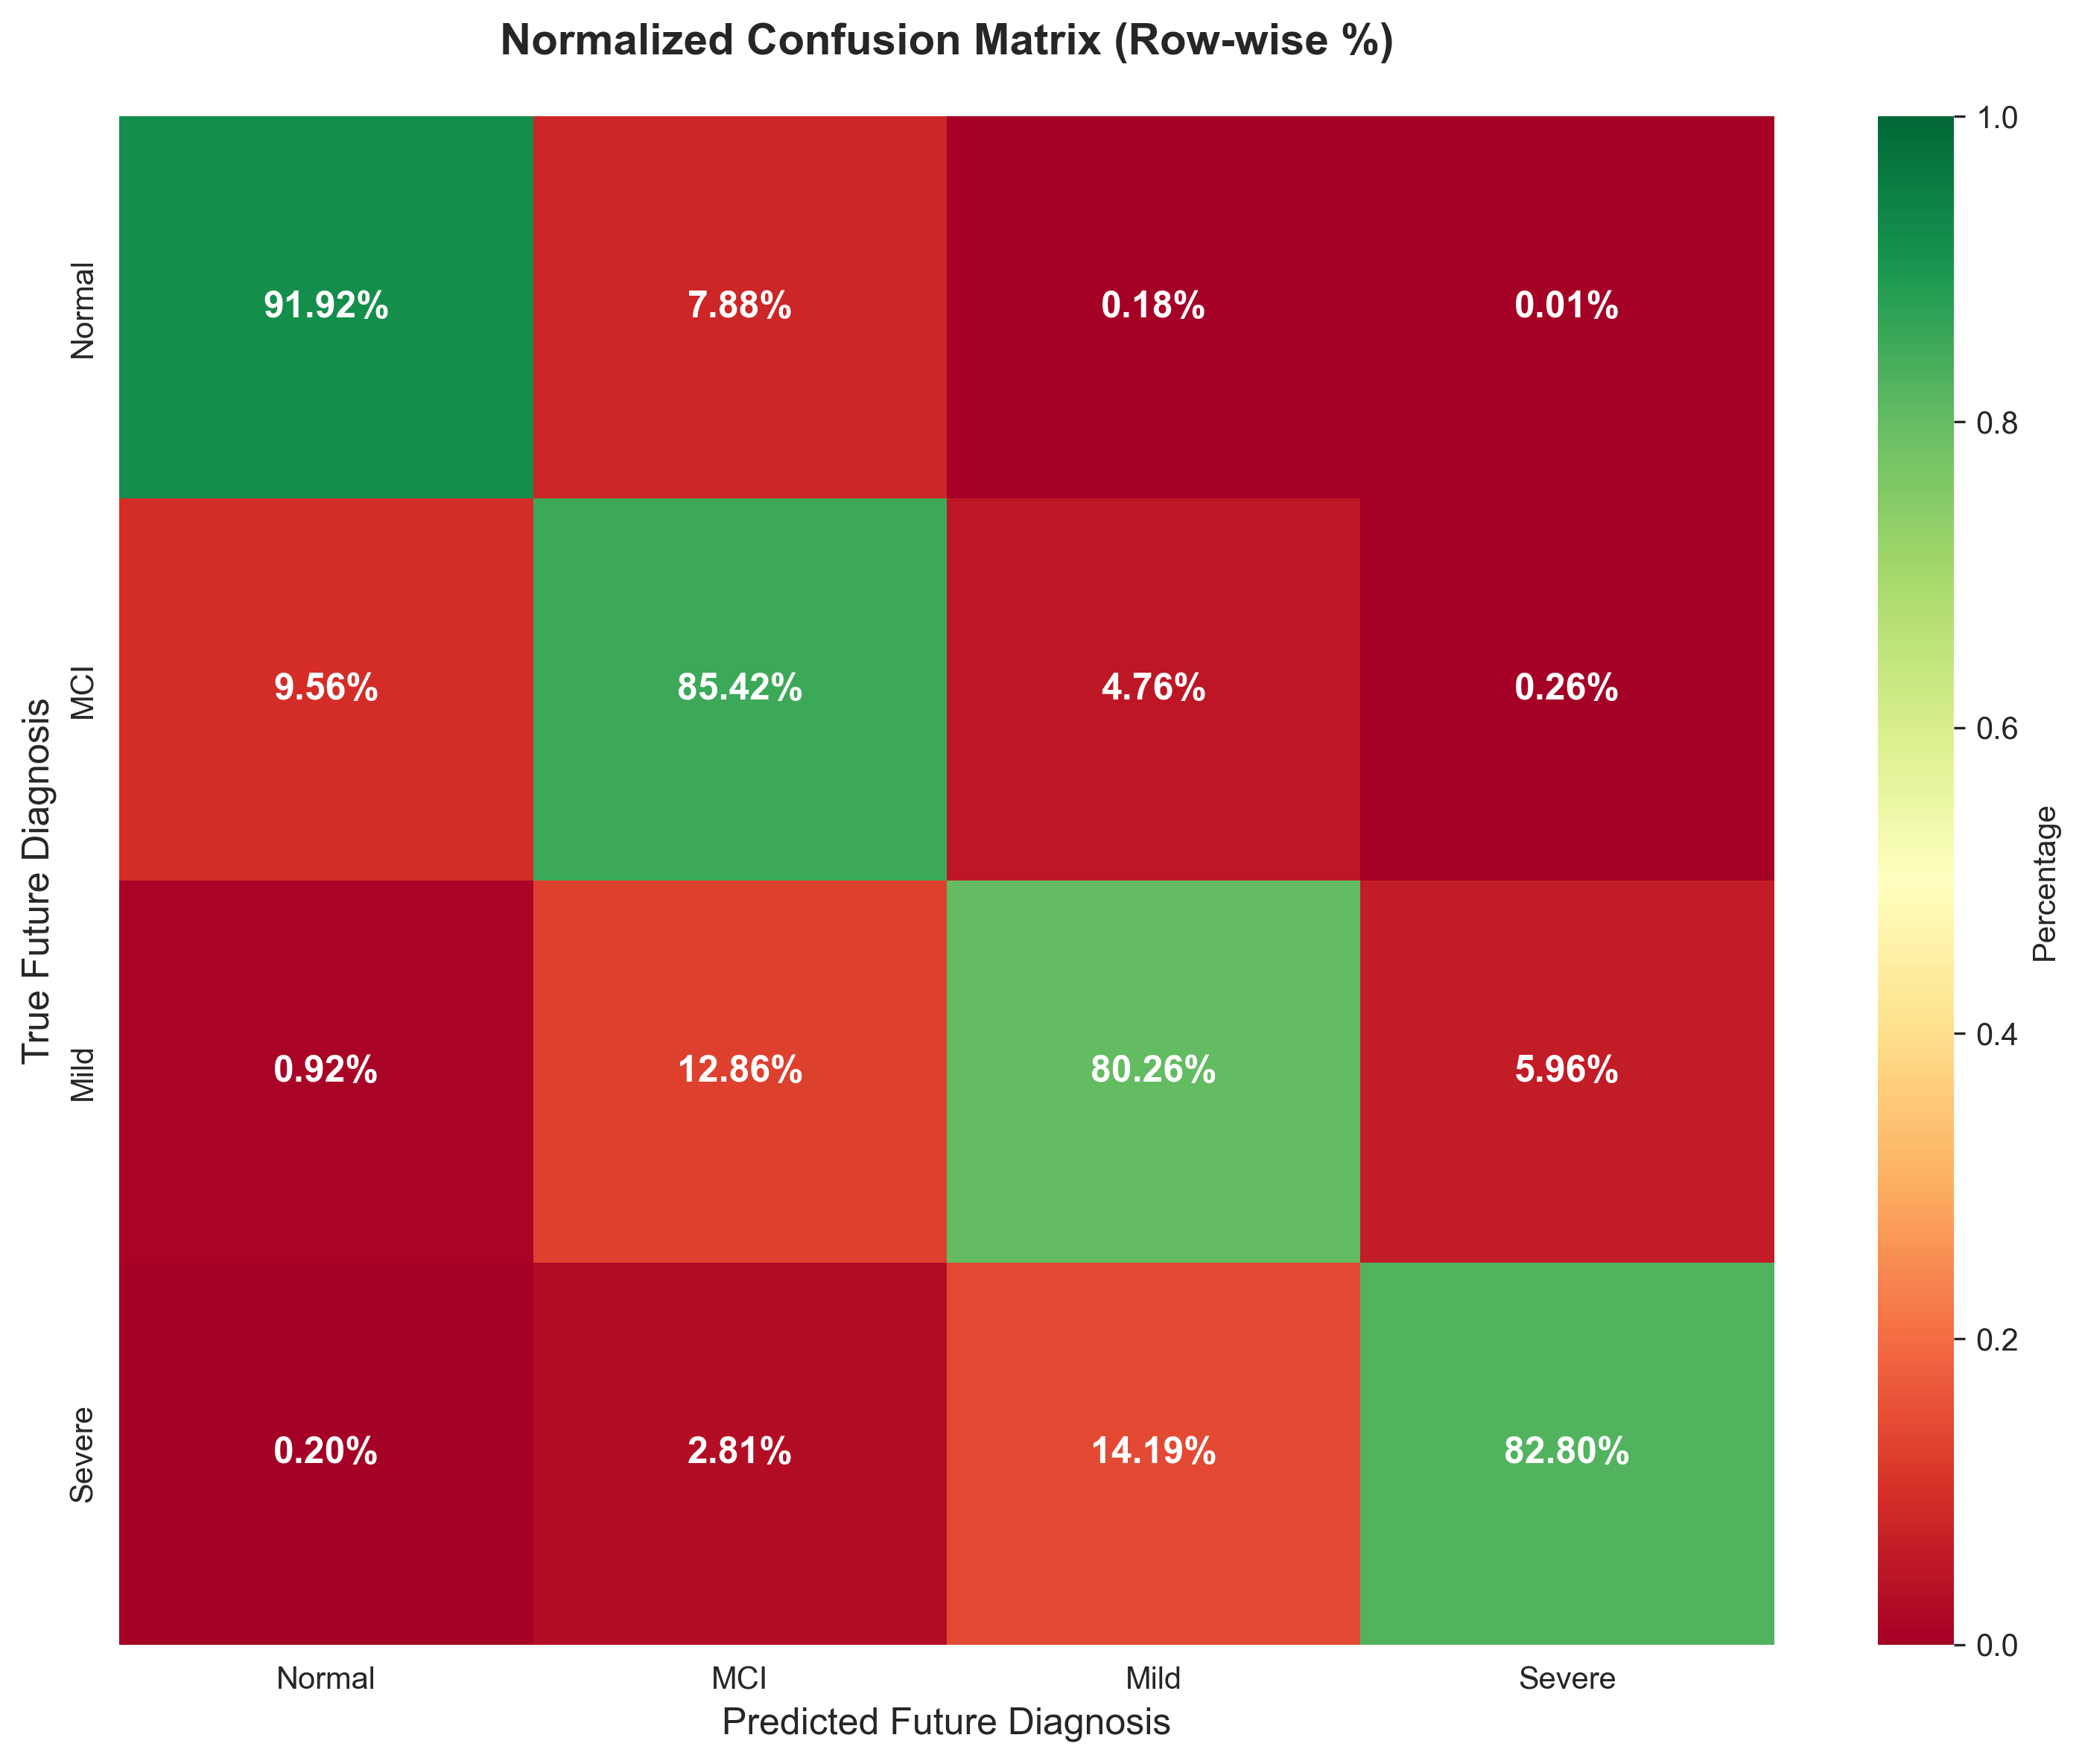
\includegraphics[width=0.62\columnwidth]{output/confusion_matrix_normalized.png}
\caption{Normalized Confusion Matrix. Diagonal elements represent recall (sensitivity) for each class. The model achieves high accuracy for `Normal' and `Severe' endpoints, with expected confusion between clinically adjacent stages (MCI/Mild).}
\label{fig:cm_norm}
\end{figure}

\subsection{Progression Trajectory Analysis}

To visualize longitudinal progression patterns, we generated a Sankey diagram (Supplementary Figure S2) mapping true diagnoses at visit $t$ to predicted diagnoses at visit $t+1$. This flow visualization confirms that the model successfully captures:
\begin{itemize}
    \item \textbf{Stability patterns:} Majority of Normal patients correctly predicted to remain Normal.
    \item \textbf{Progression events:} MCI $\rightarrow$ Mild and Mild $\rightarrow$ Severe transitions appropriately identified.
    \item \textbf{Reversion cases:} Occasional MCI $\rightarrow$ Normal predictions, reflecting clinical reality where some MCI patients stabilize.
\end{itemize}

\subsection{Ablation Study: Component Contribution Analysis}

To quantify the contribution of synthetic oversampling and model ensembling, we evaluated three configurations on the same patient-level test split. The base XGBoost model achieved 0.8782 accuracy and 0.8514 macro F1. Adding BorderlineSMOTE reduced performance to 0.8684 accuracy and 0.8376 macro F1, while the full ensemble with BorderlineSMOTE achieved 0.8584 accuracy and 0.8280 macro F1. Thus, neither added component improved aggregate performance on this split.

\subsection{Ablation Study: Comparison with Ensembles}

A critical question in clinical AI is whether increased model complexity translates to better performance. We compared our primary XGBoost framework against a complex weighted ensemble (Supplementary Table S1).

\textbf{Interpretation:} The base XGBoost model without synthetic oversampling or ensembling yielded the highest aggregate performance. Adding SMOTE reduced macro F1 by approximately 1.4 percentage points, and the full ensemble reduced it by approximately 2.3 percentage points relative to the base configuration (Supplementary Table S1). These results support a ``Frugal AI'' approach in which the simpler model is preferred for this evaluation split.

\subsection{Sensitivity Analysis: Excluding Genetic-Risk Features}
\label{sec:sensitivity}

Because many care settings do not routinely collect genetic data, we repeated the base XGBoost configuration with all 11 APOE- and family-history--derived columns removed: the five raw variables (\texttt{NACCAPOE}, \texttt{NACCNE4S}, \texttt{NACCFAM}, \texttt{NACCMOM}, \texttt{NACCDAD}), the five engineered APOE4 indicators (\texttt{apoe4\_any}, \texttt{apoe4\_double}, \texttt{apoe4\_count}, \texttt{apoe4\_age\_risk}, \texttt{apoe4\_elderly}), and the age$\times$APOE4 interaction term. This left 90 predictors. The patient-level split, preprocessing, class weights, and hyperparameters were held identical to the base configuration, so the only change was the input feature set.

\begin{table}[htbp]
\caption{Sensitivity Analysis: Base XGBoost With and Without Genetic-Risk Features}
\label{tab:sensitivity}
\begin{center}
\begin{tabular}{lccc}
\toprule
\textbf{Model} & \textbf{Accuracy} & \textbf{Macro F1} & \textbf{Weighted F1} \\
\midrule
Base (101 predictors) & 0.8782 & 0.8514 & 0.8795 \\
No genetic-risk features (90 predictors) & 0.8779 & 0.8505 & 0.8792 \\
\midrule
$\Delta$ & $-0.0003$ & $-0.0009$ & $-0.0003$ \\
\bottomrule
\end{tabular}
\end{center}
\end{table}

Removing all APOE genotype and family-history information changed accuracy by 0.03 percentage points and macro F1 by 0.09 percentage points (85.14\% to 85.05\%), with per-class F1 changing by at most 0.19 percentage points (Severe, 0.8767 to 0.8748). Performance was therefore essentially unchanged, indicating that the framework does not depend on genetic testing.

\subsection{Error Analysis and Error Severity}

We conducted a detailed analysis of the 3,646 misclassified samples (12.2\% error rate) to characterize error severity (Table~\ref{tab:errors}).

\begin{table}[htbp]
\caption{Error Severity Distribution}
\label{tab:errors}
\begin{center}
\begin{tabular}{lcc}
\toprule
\textbf{Error Severity} & \textbf{Count} & \textbf{Percentage} \\
\midrule
1 stage off (e.g., Normal $\rightarrow$ MCI) & 3,459 & 94.9\% \\
2 stages off (e.g., Normal $\rightarrow$ Mild) & 178 & 4.9\% \\
3 stages off (e.g., Normal $\rightarrow$ Severe) & 9 & 0.2\% \\
\bottomrule
\end{tabular}
\end{center}
\end{table}

\textbf{Clinical Interpretation:} The overwhelming majority (94.9\%) of errors are ``1-stage off,'' meaning predictions remain clinically adjacent to ground truth. Errors 3 stages off comprised 0.2\% of misclassifications.

The top confusion patterns were:
\begin{itemize}
    \item Normal $\rightarrow$ MCI: 1,189 cases (7.9\%)
    \item MCI $\rightarrow$ Normal: 769 cases (9.6\%)
    \item Severe $\rightarrow$ Mild: 505 cases (14.2\%)
\end{itemize}

These patterns align with clinical reality, where diagnostic boundaries between adjacent stages are inherently ambiguous. Class-specific error rates are shown in Supplementary Figure S4.

\textbf{Confidence Calibration:} The average maximum predicted probability was 0.893 for correct predictions and 0.737 for incorrect predictions, a difference of 0.156.

\subsection{Demographic Fairness Analysis}

A critical requirement for clinical AI is equitable performance across demographic subgroups. We evaluated the model's fairness across Sex, Age, and Race (Table~\ref{tab:fairness}; Figure~\ref{fig:fairness}).

\begin{table}[htbp]
\caption{Fairness Analysis: Performance by Demographic Subgroup}
\label{tab:fairness}
\begin{center}
\begin{tabular}{lccc}
\toprule
\textbf{Group} & \textbf{N} & \textbf{Accuracy} & \textbf{F1-Macro} \\
\midrule
\multicolumn{4}{l}{\textit{By Sex}} \\
Male & 12,683 & 0.868 & 0.854 \\
Female & 17,256 & 0.886 & 0.846 \\
\midrule
\multicolumn{4}{l}{\textit{By Age Group}} \\
$<$65 years & 5,243 & 0.900 & 0.866 \\
65--74 years & 10,696 & 0.898 & 0.863 \\
75--84 years & 10,424 & 0.861 & 0.844 \\
85+ years & 3,576 & 0.838 & 0.824 \\
\midrule
\multicolumn{4}{l}{\textit{By Race}} \\
White & 24,826 & 0.880 & 0.853 \\
Black/African American & 3,723 & 0.875 & 0.836 \\
Asian & 791 & 0.850 & 0.818 \\
American Indian/Alaska Native & 190 & 0.853 & 0.803 \\
Native Hawaiian/Pacific Islander & 13 & 0.923 & 0.894 \\
Other/Multiracial & 286 & 0.874 & 0.865 \\
Unknown & 110 & 0.873 & 0.851 \\
\bottomrule
\end{tabular}
\end{center}
\end{table}

\textbf{Key Findings:}
\begin{itemize}
    \item \textbf{Sex:} Male and female F1-macro scores were 0.854 and 0.846, respectively.
    \item \textbf{Age:} Performance was lowest in the 85+ cohort (F1=0.824) and highest in the $<$65 cohort (F1=0.866), reflecting increased diagnostic complexity among the oldest participants.
    \item \textbf{Race:} F1-macro ranged from 0.803 (American Indian/Alaska Native) to 0.894 (Native Hawaiian/Pacific Islander). Race code 99 was retained and reported as Unknown rather than dropped. Small subgroup sizes require cautious interpretation; in particular, the Native Hawaiian/Pacific Islander estimate ($N=13$) should not be interpreted as meaningful evidence of fairness or unfairness in either direction.
\end{itemize}

\subsection{Feature Importance and Interpretability}

To enable clinical transparency, we applied SHAP TreeExplainer to quantify feature contributions (Figure~\ref{fig:shap}, Table~\ref{tab:shap}).

\begin{figure}[htbp]
\centering
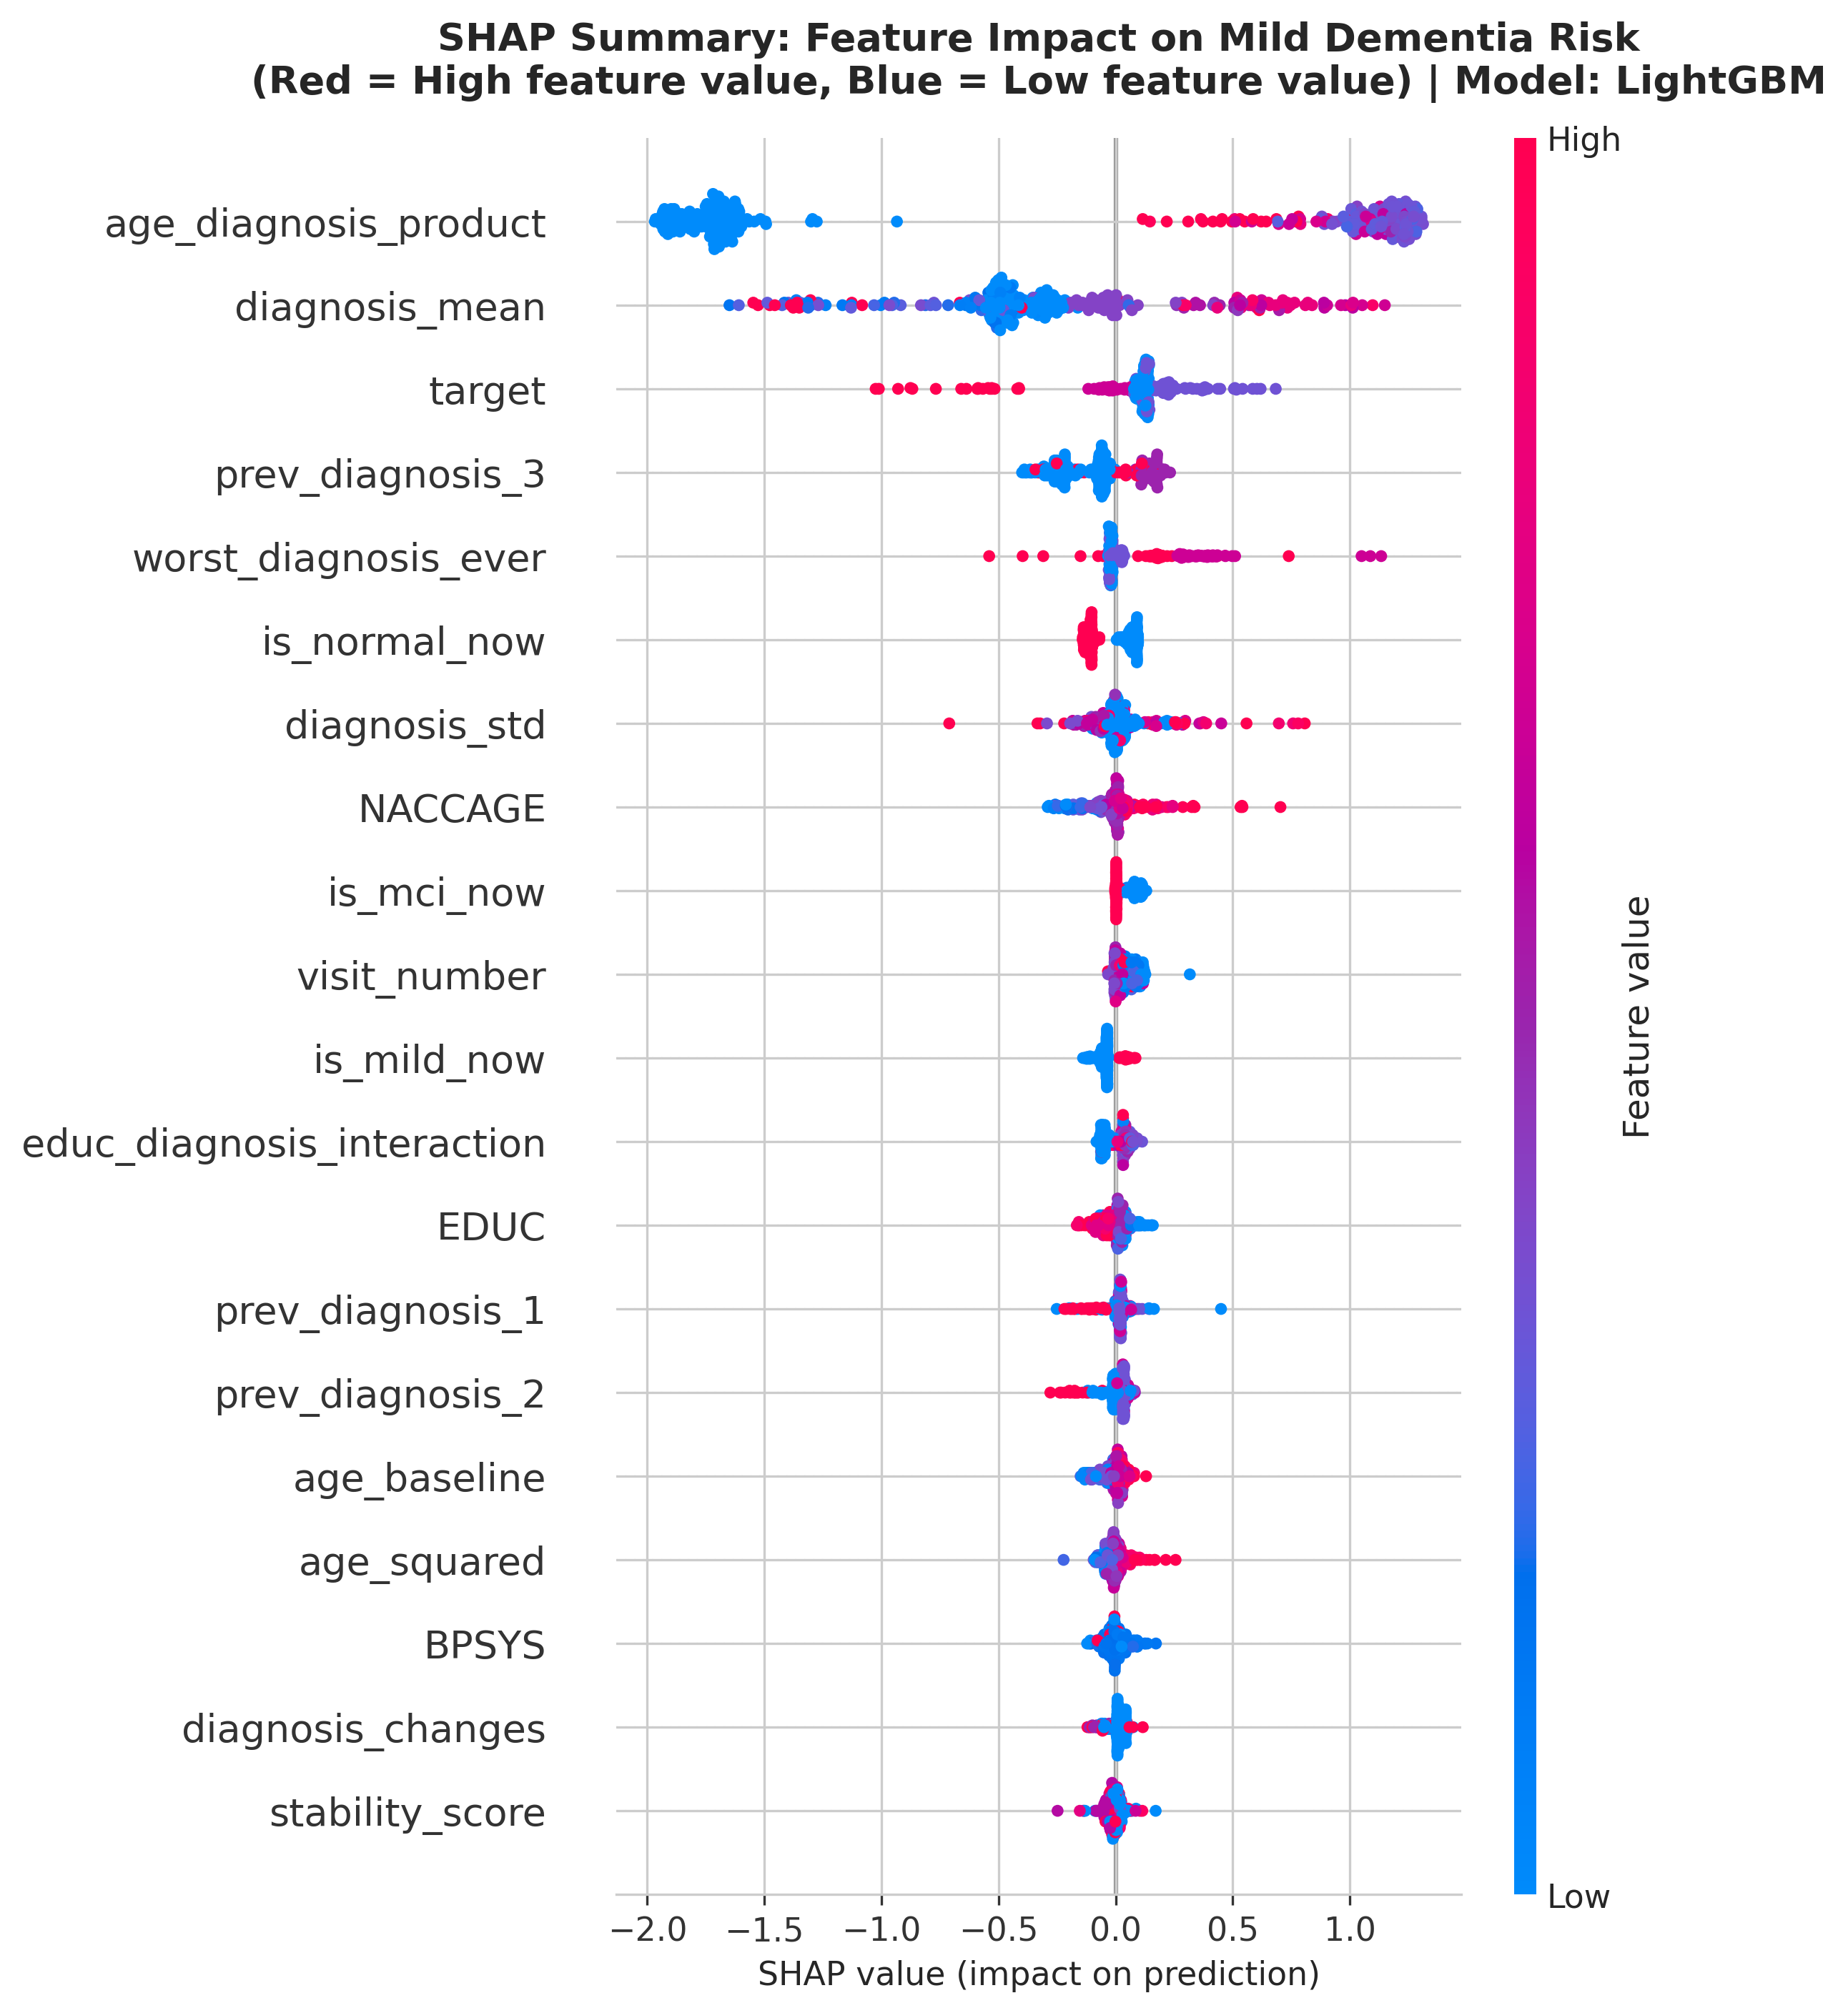
\includegraphics[width=0.68\columnwidth]{output/shap_beeswarm.png}
\caption{SHAP Beeswarm Plot. Features are ranked by global importance. Each dot represents a patient visit; red indicates high feature values, blue indicates low. Horizontal spread shows impact magnitude on predictions.}
\label{fig:shap}
\end{figure}

\begin{table}[H]
\caption{Top 5 SHAP Features by Diagnostic Class}
\label{tab:shap}
\begin{center}
\footnotesize
\resizebox{\textwidth}{!}{%
\begin{tabular}{clllll}
\toprule
\textbf{Rank} & \textbf{Normal} & \textbf{MCI} & \textbf{Mild} & \textbf{Severe} \\
\midrule
1 & \texttt{diagnosis\_mean} & \texttt{diagnosis\_mean} & \texttt{age\_diagnosis\_product} & \texttt{age\_diagnosis\_product} \\
2 & target (current) & \texttt{diagnosis\_std} & \texttt{diagnosis\_mean} & target (current) \\
3 & \texttt{age\_diagnosis\_product} & \texttt{diagnosis\_changes} & \texttt{worst\_diagnosis\_ever} & \texttt{diagnosis\_std} \\
4 & \texttt{diagnosis\_std} & target (current) & \texttt{is\_mild\_now} & \texttt{diagnosis\_mean} \\
5 & \texttt{diagnosis\_changes} & \texttt{worst\_diagnosis\_ever} & target (current) & \texttt{educ\_diagnosis\_interaction} \\
\bottomrule
\end{tabular}%
}
\end{center}
\end{table}

\textbf{Clinical Interpretation:}
\begin{itemize}
    \item \textbf{Diagnosis Trajectory Features} (particularly \texttt{diagnosis\_mean}, \texttt{diagnosis\_std}, and \texttt{diagnosis\_changes}) dominate predictions, confirming that longitudinal disease history is highly informative for prognosis.
    \item \textbf{Age-Diagnosis Interactions} (\texttt{age\_diagnosis\_product}) are important predictors, capturing progression risk in older patients with existing cognitive impairment.
    \item \textbf{Current Diagnostic State} (\texttt{target} and \texttt{is\_mild\_now}) provides strong baseline information for prognosis.
\end{itemize}

Class-specific feature comparisons and the mean-absolute-SHAP bar chart are provided in Supplementary Figures S5 and S6.

\subsection{ROC Curve Analysis}

Multi-class ROC curves (Figure~\ref{fig:roc}) demonstrate strong discriminative performance, with AUC values of 0.979, 0.952, 0.967, and 0.989 for Normal, MCI, Mild, and Severe classes, respectively.

\begin{figure}[htbp]
\centering
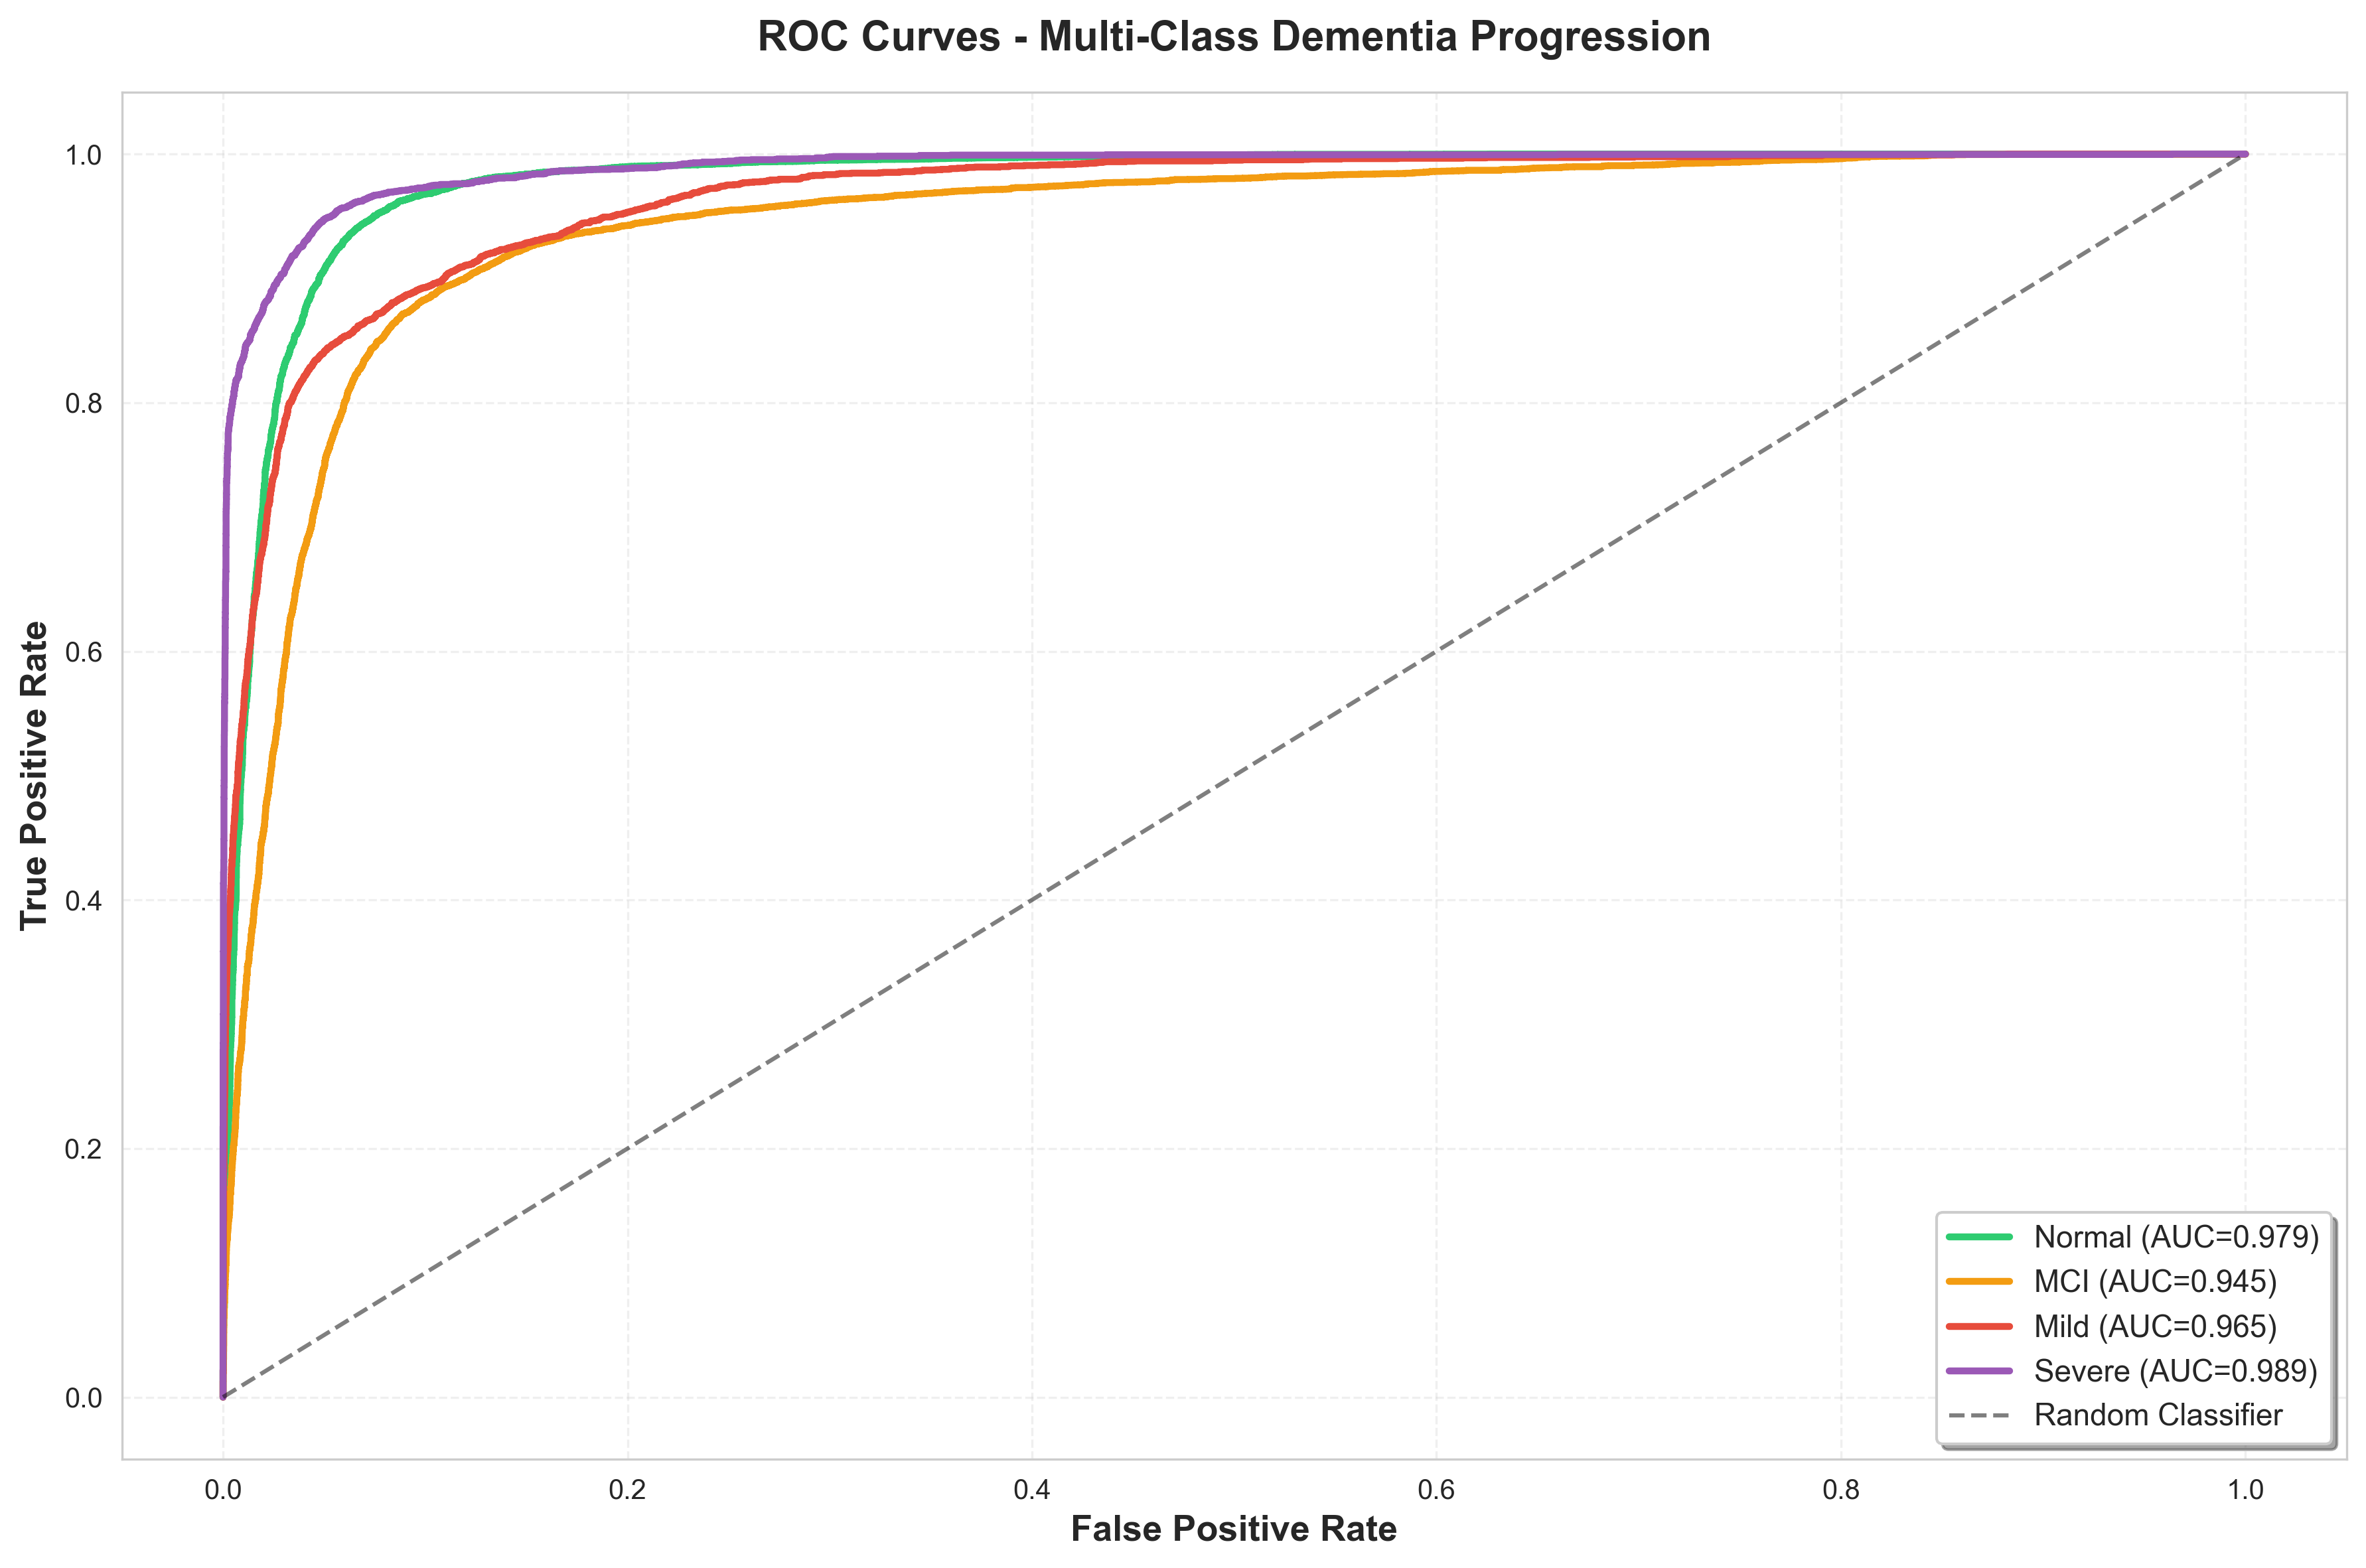
\includegraphics[width=0.6\columnwidth]{output/roc_curves.png}
\caption{Multi-class ROC Curves. AUC values are 0.979 for Normal, 0.952 for MCI, 0.967 for Mild, and 0.989 for Severe.}
\label{fig:roc}
\end{figure}

\begin{figure}[htbp]
\centering
\begin{subfigure}{0.48\textwidth}
\centering
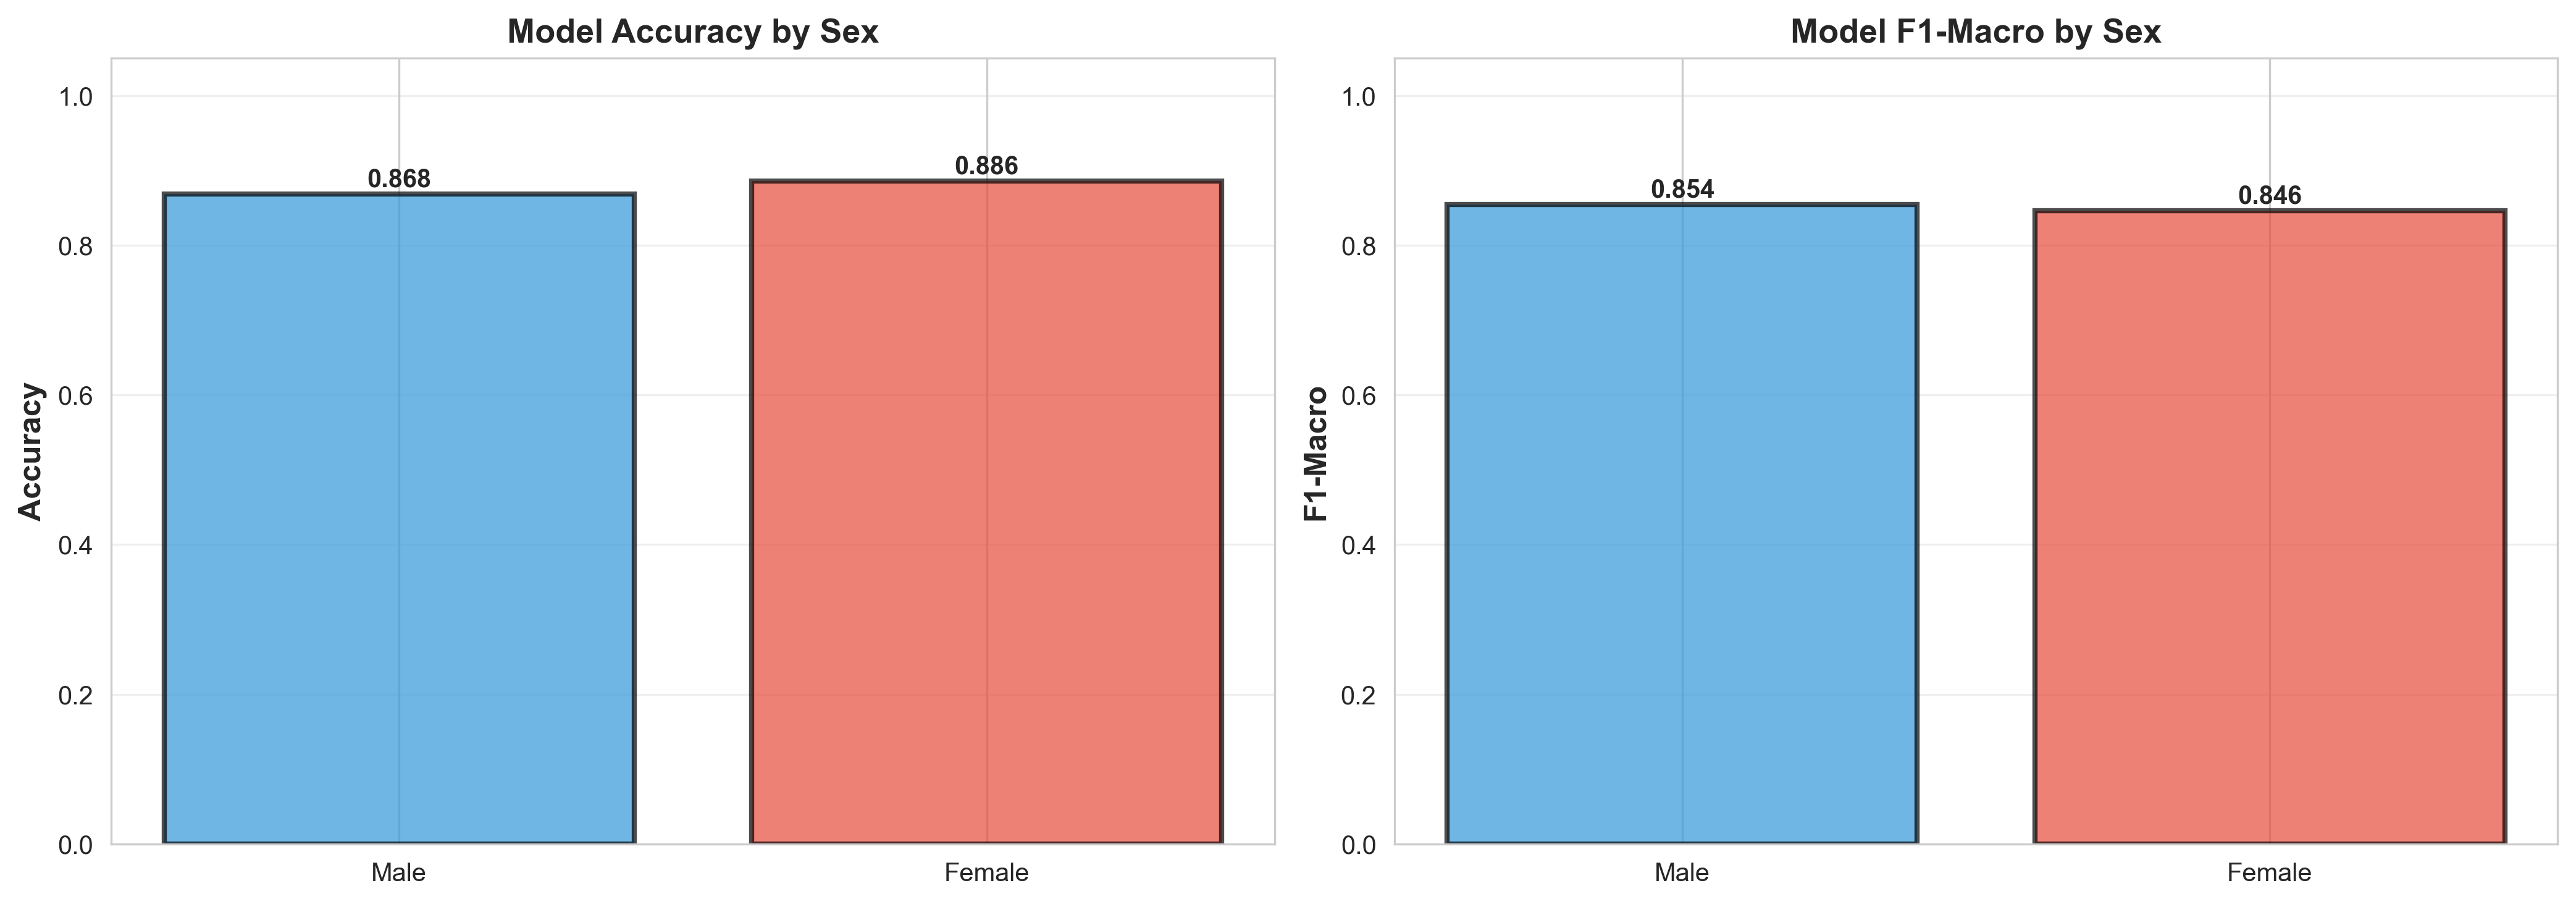
\includegraphics[width=\linewidth]{output/fairness_by_sex.png}
\caption{Sex}
\end{subfigure}
\hfill
\begin{subfigure}{0.48\textwidth}
\centering
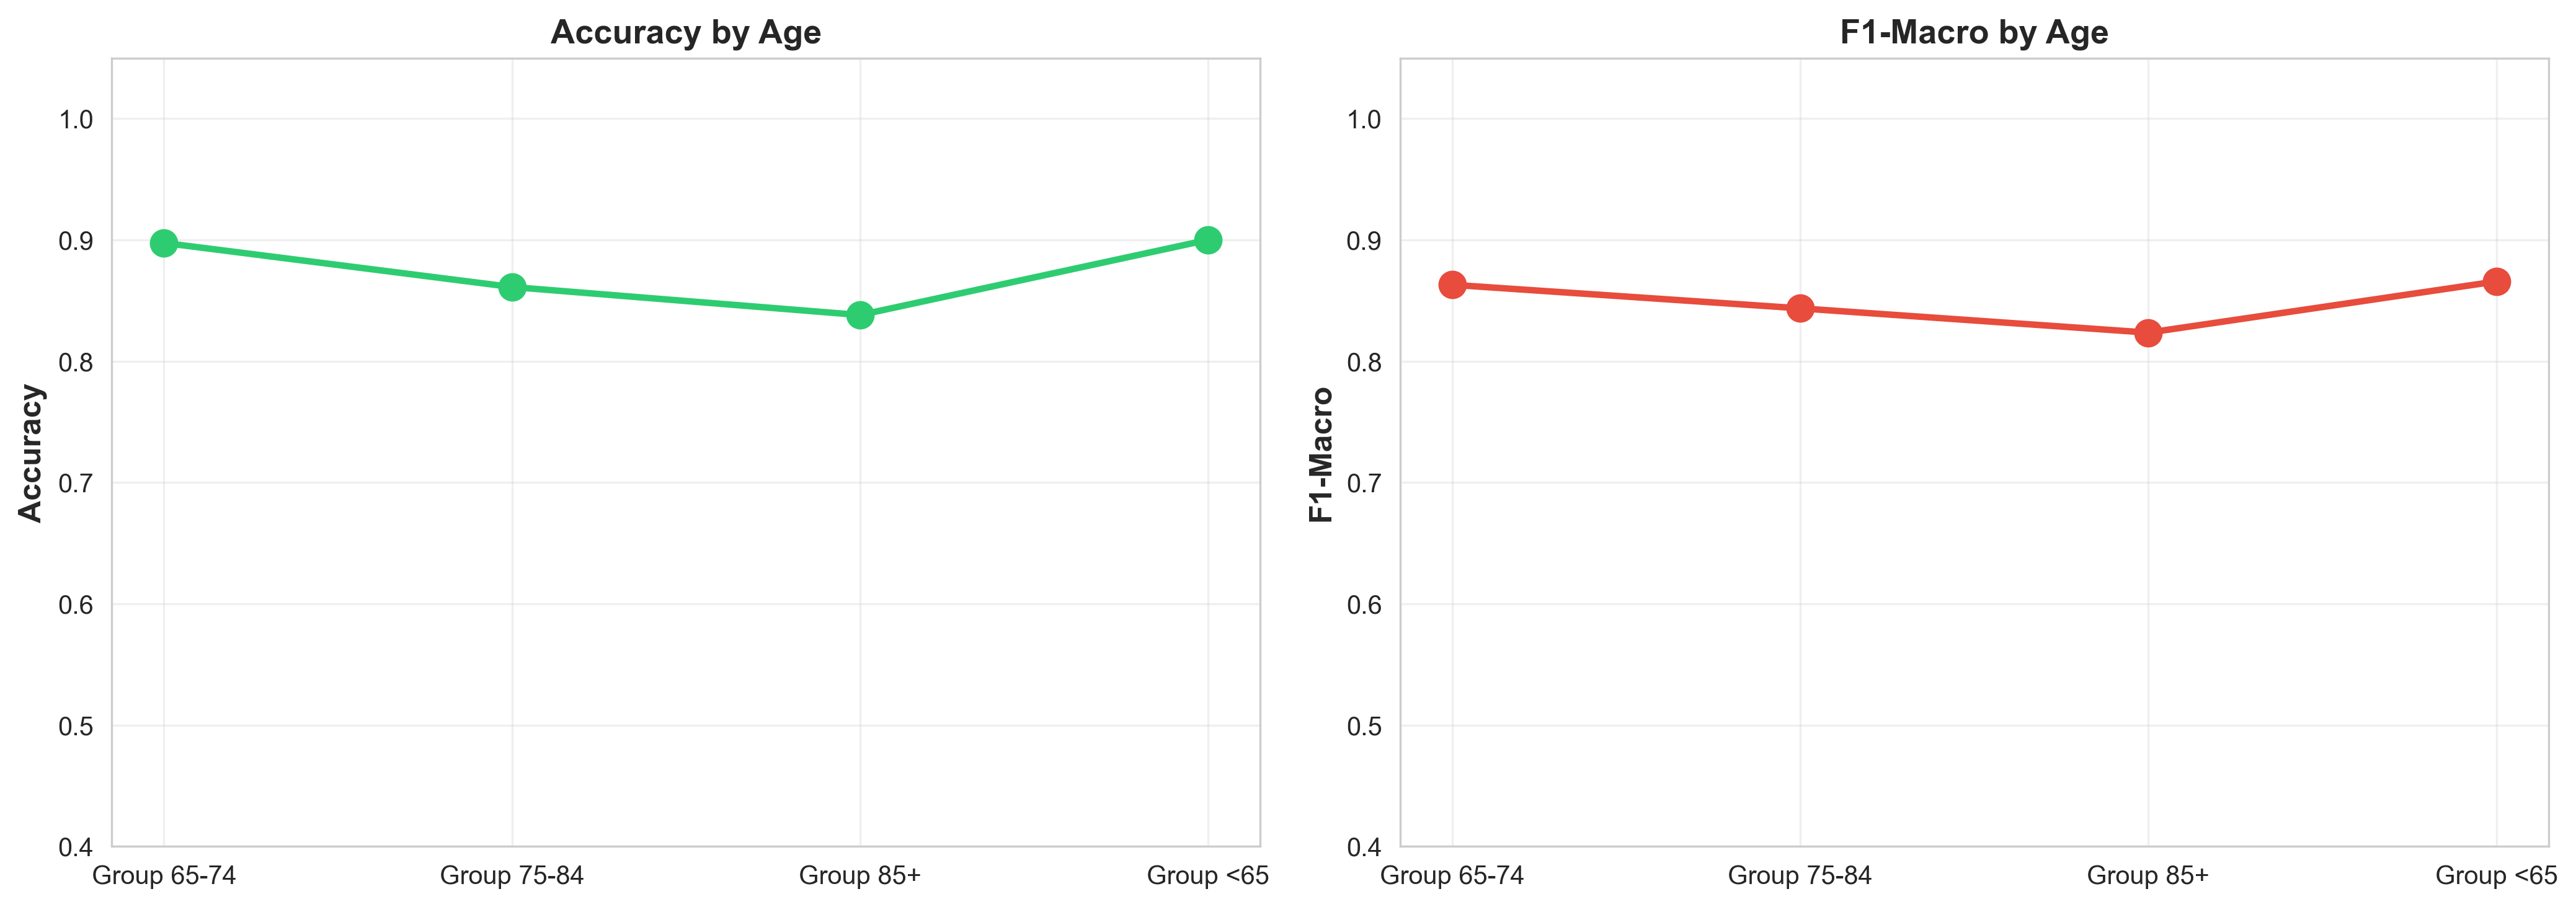
\includegraphics[width=\linewidth]{output/fairness_by_age.png}
\caption{Age}
\end{subfigure}
\caption{Fairness Analysis by Sex (a) and Age (b).}
\label{fig:fairness}
\end{figure}

\subsection{Model Calibration and Confidence Analysis}

For clinical deployment, predicted probabilities must accurately reflect true outcome likelihoods, and calibration is widely regarded as a critical failure mode of predictive models~\cite{vancalster2019}. We evaluated calibration using reliability diagrams (Supplementary Figure S7) and the expected calibration error (ECE) metric~\cite{guo2017}. After correcting the probability-normalization step, the calibration ECE values are 0.127, 0.036, 0.099, and 0.046 for Normal, MCI, Mild, and Severe, respectively. Three of the four classes are well calibrated (ECE below 0.1); Normal remains moderately calibrated. Given the improvement already achieved relative to the initial model, we did not pursue further post-hoc calibration, as an additional retraining cycle for a marginal gain on one class would run counter to the simplicity the model is intended to demonstrate.

Confidence distributions are shown in Supplementary Figure S8; correct predictions have mean maximum probability 0.893 versus 0.737 for incorrect predictions.

% =================================================================================
% 4. DISCUSSION
% =================================================================================
\section{Discussion}

\subsection{Clinical Implications}

This study demonstrates that robust dementia progression prediction is achievable using exclusively routine clinical data, without reliance on expensive neuroimaging or invasive biomarker assays.

The clinical-only approach addresses the critical \textbf{accessibility gap} in current AI solutions. While MRI/PET-based models may achieve marginally higher accuracy in research settings, they cannot scale to population-level screening in primary care, community health centers, or resource-limited settings where the majority of dementia patients first present. Our framework enables:

\begin{itemize}
    \item \textbf{Primary Care Deployment:} Integration with electronic health record systems for automated risk stratification during routine visits.
    \item \textbf{Resource-Limited Settings:} Applicability in low- and middle-income countries where neuroimaging infrastructure is unavailable.
    \item \textbf{Population Screening:} Cost-effective identification of high-risk individuals for targeted intervention.
\end{itemize}

\subsection{Error Severity Analysis}

Beyond aggregate accuracy, our error severity analysis provides crucial insights for clinical deployment: a Normal patient misclassified as MCI receives monitoring rather than false reassurance, a Severe patient misclassified as Mild still receives dementia care, and catastrophic Normal $\leftrightarrow$ Severe misclassifications are exceedingly rare.

This error profile is far preferable to models that achieve higher accuracy by confidently classifying boundary cases, only to fail catastrophically on a small fraction of patients.

\subsection{Algorithmic Fairness}

Performance was broadly similar across the evaluated demographic subgroups, although limited sample sizes in several racial groups (e.g., N=13 for Native Hawaiian/Pacific Islander, N=190 for American Indian/Alaska Native) prevent definitive conclusions regarding algorithmic fairness for those groups~\cite{rajkomar2018,gianfrancesco2018}.

\subsection{Feature Interpretability}

We note that the model is an intentionally autoregressive next-visit stage forecaster: it uses the patient's own diagnostic history as predictors (consistent with the SHAP findings in Table~\ref{tab:shap}), which differs from predicting the onset of underlying neuropathological change, while still being clinically useful for anticipating the next recorded CDR-based stage.

SHAP analysis identifies clinically meaningful predictors. The dominance of longitudinal diagnosis trajectory features (\texttt{diagnosis\_mean}, \texttt{worst\_diagnosis\_ever}) confirms that disease history---the pattern of cognitive decline over time---is more prognostically informative than any single biomarker measurement. This finding aligns with clinical intuition and supports the value of longitudinal follow-up in dementia care.

The emergence of age-diagnosis interactions as strong predictors validates known epidemiological relationships: cognitive impairment in older patients carries higher progression risk than equivalent impairment in younger patients. This non-linear interaction effect would be missed by simpler linear models.

\subsection{Clinical Translation Roadmap}

Translation would begin with a silent-mode EHR integration in primary-care and community-screening settings. At each eligible visit, the system would retrieve routinely available predictors, apply the locked preprocessing and base XGBoost model, and return a calibrated stage-risk summary with an uncertainty flag to the clinician; no autonomous diagnosis or treatment decision would be made. The interface should display current inputs, predicted next-visit stage, and a concise explanation, while recording model version, timestamp, overrides, and referral actions for auditability.

Prospective validation should first assess technical transportability across sites, temporal drift, calibration, subgroup performance, missing-data behavior, and referral thresholds before any patient-facing alert is enabled, consistent with current reporting and validation guidance for machine-learning prediction models~\cite{collins2024}. A follow-on implementation study should measure workflow fit, alert burden, usability, adoption, time to specialist referral, clinician override patterns, equity of access, safety events, and changes in appropriate diagnostic work-up. It should also test whether model-supported referral improves clinically meaningful outcomes without increasing unnecessary testing. These staged evaluations would convert this retrospective proof of concept into a monitored clinical decision-support pathway in primary-care and community contexts.

\subsection{Comparison with Neuroimaging Models}

While MRI-based deep learning models often achieve 90--95\% accuracy in binary tasks, direct comparison is limited because our four-class next-visit prediction is more challenging and the heterogeneous NACC cohort differs from homogeneous imaging cohorts. Clinical features may generalize more readily across institutions than scanner-sensitive imaging features, while requiring no additional testing cost and supporting first-line screening.

We propose that clinical-only and imaging-based approaches are complementary rather than competing. Our model can serve as a first-line screening tool, with imaging reserved for borderline cases or therapeutic decision-making requiring precise anatomical information.

\subsection{Limitations and Future Work}

Several limitations merit consideration:

\begin{enumerate}
    \item \textbf{Dataset Bias:} The NACC cohort, while large and multi-center, is collected from specialized Alzheimer's research centers and may not fully reflect primary care populations. External validation on community-based cohorts is needed.

    \item To assess population comparability with an external cohort, we compared baseline demographic and APOE epsilon4 distributions between NACC (n=37,633) and the Alzheimer's Disease Neuroimaging Initiative (ADNI; n=2,049). Of our 101 predictors, only sex, race, ethnicity, age, and APOE epsilon4 carrier count had directly comparable fields in the public ADNIMERGE table; the comorbidity, functional, and behavioral variables that make up most of our feature set are not captured in ADNIMERGE, which is built around cognitive testing and imaging/biomarker measures rather than the detailed medical-history assessment used in NACC's UDS. Even restricted to these comparable fields, the cohorts differ appreciably: ADNI was less racially diverse (92.7\% White vs. 80.9\% in NACC) and had a lower proportion of Hispanic/Latino participants (3.2\% vs. 8.1\%), consistent with ADNI's research/clinical-trial recruitment relative to NACC's clinic-based ADRC population. Additionally, ADNI's diagnostic categorization does not map directly onto the CDR-Global-based staging used here, precluding outcome-level comparison even where demographic fields align. Given this limited feature overlap, we did not attempt a reduced-feature model comparison against ADNI, as it would not constitute a meaningful external validation of the full model; genuine external validation will require a cohort with comparably detailed clinical and comorbidity data~\cite{petersen2010,aisen2024}.

    \item \textbf{Minority Representation:} Sample sizes for some racial groups (American Indian/Alaska Native, Native Hawaiian/Pacific Islander) are limited, necessitating cautious interpretation of fairness metrics for these populations.

    \item \textbf{Temporal Prediction Horizon:} We predict next-visit diagnosis, but the time interval between visits in the NACC cohort is variable, ranging from months to years depending on participant scheduling and retention. This variability is not explicitly modeled in the current framework; the model treats all next-visit predictions equivalently regardless of the elapsed time between assessments. Future work will adopt survival analysis approaches---such as Cox-Time or DeepSurv---to explicitly model variable time horizons and predict time-to-conversion rather than next-visit state alone.

    \item \textbf{Feature Availability and Oversampling:} APOE4 genotyping may not be routinely available, and BorderlineSMOTE may generate biologically implausible combinations; sensitivity analysis under feature missingness and cost-sensitive alternatives warrant further study.
\end{enumerate}

Future work will include: (1) external validation on the Alzheimer's Disease Neuroimaging Initiative (ADNI) cohort, (2) survival analysis for time-to-conversion prediction, (3) integration with electronic health record systems for prospective validation, and (4) development of a clinical decision support interface for end-user deployment.

% =================================================================================
% 5. CONCLUSION
% =================================================================================
\section{Conclusion}

We presented a robust and interpretable machine learning framework for predicting dementia progression using exclusively routine clinical data. The base XGBoost model achieved 87.82\% accuracy, 85.14\% macro F1-score, and 87.95\% weighted F1-score on a large, multi-center cohort. Ablation analysis showed that adding SMOTE or a more complex ensemble reduced aggregate performance on this split, supporting a ``Frugal AI'' deployment strategy.

The framework's key strengths include:
\begin{itemize}
    \item \textbf{Clinical-Only Input:} No imaging or CSF testing is required, and the framework does not depend on genetic testing: excluding APOE genotype and family-history variables changed macro F1 by only 0.09 percentage points (Section~\ref{sec:sensitivity}).
    \item \textbf{Rigorous Validation:} Patient-level data splitting prevents information leakage and ensures honest performance estimates.
    \item \textbf{Fairness:} Performance was broadly similar across the evaluated sex, age, and racial subgroups, though small subgroup sizes (e.g., N=13 Native Hawaiian/Pacific Islander, N=190 American Indian/Alaska Native) preclude definitive fairness conclusions for those groups.
    \item \textbf{Interpretability:} SHAP-based feature attribution enables clinician understanding and regulatory compliance.
    \item \textbf{Error Severity:} Error severity analysis shows that most misclassifications remain clinically proximal (94.9\% one stage off), although this does not by itself establish clinical safety absent a prospective decision-impact study.
\end{itemize}

This work supports a ``Frugal AI'' paradigm, democratizing access to early Alzheimer's detection in resource-constrained environments and bridging the gap between theoretical AI advances and practical clinical tools.

% =================================================================================
% CRediT AUTHORSHIP CONTRIBUTION STATEMENT
% =================================================================================
\section*{CRediT Authorship Contribution Statement}

\textbf{MD Walid Waccub Swadhin:} Conceptualization, Methodology, Software, Formal analysis, Data Curation, Writing -- Original Draft, Visualization.

% =================================================================================
% ACKNOWLEDGMENTS
% =================================================================================
\section*{Acknowledgments}
We thank the participants and clinical staff at the Alzheimer's Disease Research Centers (ADRCs) for their contributions to dementia research. The content is solely the responsibility of the authors and does not necessarily represent the official views of the National Institutes of Health.

The NACC database is funded by NIA/NIH Grant U24 AG072122. NACC data are contributed by the NIA-funded ADRCs: P30 AG062429 (PI James Brewer, MD, PhD), P30 AG066468 (PI Oscar Lopez, MD), P30 AG062421 (PI Teresa Gomez-Isla, MD), P30 AG066509 (PI Thomas Grabowski, MD), P30 AG066514 (PI Mary Sano, PhD), P30 AG066530 (PI Helena Chui, MD, Arthur Toga, PhD), P30 AG066507 (PI Marilyn Albert, PhD), P30 AG066444 (PI David Holtzman, MD), P30 AG066518 (PIs Lisa Silbert, MD, Kevin Duff, PhD), P30 AG066512 (PI Thomas Wisniewski, MD), P30 AG066462 (PI Scott Small, MD), P30 AG072979 (PI David Wolk, MD), P30 AG072972 (PIs Charles DeCarli, MD, Rachel Whitmer, PhD), P30 AG072976 (PI Andrew Saykin, PsyD), P30 AG072975 (PI Julie Schneider, MD, MS), P30 AG072978 (PI Ann McKee, MD), P30 AG072977 (PI Robert Vassar, PhD), P30 AG066519 (PI Joshua Grill, PhD), P30 AG062677 (PIs Brad Boeve, MD, Ronald Petersen, MD, PhD), P30 AG079280 (PI Jessica Langbaum, PhD), P30 AG062422 (PI Gil Rabinovici, MD), P30 AG066511 (PI Allan Levey, MD, PhD), P30 AG072946 (PI Linda Van Eldik, PhD), P30 AG062715 (PI Sanjay Asthana, MD, FRCP), P30 AG072973 (PI Russell Swerdlow, MD), P30 AG066506 (PIs Glenn Smith, PhD, ABPP, David Lowenstein, PhD, Ranjan Duara, MD), P30 AG066508 (PIs Stephen Strittmatter, MD, PhD, Christopher Van Dyck, MD), P30 AG066515 (PI Victor Henderson, MD, MS), P30 AG072947 (PI Suzanne Craft, PhD), P30 AG072931 (PI Henry Paulson, MD, PhD), P30 AG066546 (PIs Sudha Seshadri, MD, Gladys Maestre, MD, PhD), P30 AG086401 (PI Erik Roberson, MD, PhD), P30 AG086404 (PI Gary Rosenberg, MD), P30 AG086403 (PI Angela Jefferson, PhD), P30 AG072958 (PIs Heather Whitson, MD, Gwenn Garden, MD, PhD), P30 AG072959 (PI Jagan Pillai, MD, PhD), P30 AG092752 (Ihab Hajjar, MD, MS).

\section*{Data Availability Statement}
The NACC dataset is available through application to the National Alzheimer's Coordinating Center (https://naccdata.org/). Data used in this study reflect the September 2025 NACC data freeze (Data Request \#16386). The complete source code, trained model pipeline, and reproducibility materials for this study are publicly available at https://github.com/walidsw/nacc-dementia-progression-ai

\section*{Conflicts of Interest}
The authors declare no conflicts of interest.

\section*{Ethics Statement}
This study used de-identified secondary data from the National Alzheimer's Coordinating Center (NACC) Uniform Data Set. No new participant recruitment, direct participant contact, intervention, or identifiable-data collection was undertaken by the authors; therefore, additional institutional review board approval was not required for this analysis. The original contributing Alzheimer's Disease Research Centers obtained institutional review board approval and informed consent under their respective protocols. The analysis was conducted under the NACC Data Use Agreement associated with Data Request \#16386 (September 2025 UDS data freeze).

\section*{Funding}
Funding: This research received no specific grant from funding agencies in the public, commercial, or not-for-profit sectors. The NACC database is supported by NIA/NIH Grant U24 AG072122; that database support was not direct funding of this study.

\section*{Role of the Sponsor}
NIA/NACC had no role in the study design, analysis, interpretation of results, manuscript preparation, or decision to submit the manuscript.

\section*{Declaration of Generative AI and AI-assisted Technologies}
During manuscript preparation, the authors used GitHub Copilot and ChatGPT for language organization, drafting assistance, and code/document organization. The authors reviewed and edited all AI-assisted content, verified the reported results against the analysis outputs, and take full responsibility for the final manuscript.

% =================================================================================
% REFERENCES
% =================================================================================
\bibliographystyle{elsarticle-num}

\begin{thebibliography}{00}

\bibitem{alz2024} Alzheimer's Association, ``2024 Alzheimer's disease facts and figures,'' \textit{Alzheimer's \& Dementia}, vol. 20, no. 5, pp. 3708--3821, 2024.

\bibitem{obermeyer2019} Z. Obermeyer et al., ``Dissecting racial bias in an algorithm used to manage the health of populations,'' \textit{Science}, vol. 366, no. 6464, pp. 447--453, 2019.

\bibitem{nacc2022} National Alzheimer's Coordinating Center, ``NACC Uniform Data Set (UDS) Coding Guidebook,'' Seattle, WA, 2022.

\bibitem{chen2016} T. Chen and C. Guestrin, ``XGBoost: A Scalable Tree Boosting System,'' in \textit{Proc. 22nd ACM SIGKDD}, pp. 785--794, 2016.

\bibitem{ke2017} G. Ke et al., ``LightGBM: A Highly Efficient Gradient Boosting Decision Tree,'' in \textit{NeurIPS}, pp. 3146--3154, 2017.

\bibitem{prokhorenkova2018} L. Prokhorenkova et al., ``CatBoost: unbiased boosting with categorical features,'' in \textit{NeurIPS}, pp. 6638--6648, 2018.

\bibitem{han2005} H. Han et al., ``Borderline-SMOTE: A new over-sampling method in imbalanced data sets learning,'' in \textit{Advances in Intelligent Computing}, pp. 878--887, 2005.

\bibitem{lundberg2017} S. M. Lundberg and S.-I. Lee, ``A unified approach to interpreting model predictions,'' in \textit{NeurIPS}, pp. 4765--4774, 2017.

\bibitem{petersen2010} R. C. Petersen et al., ``Alzheimer's Disease Neuroimaging Initiative (ADNI): Clinical characterization,'' \textit{Neurology}, vol. 74, no. 3, pp. 201--209, 2010.

\bibitem{aisen2024} P. S. Aisen et al., ``The Alzheimer's Disease Neuroimaging Initiative Clinical Core,'' \textit{Alzheimer's \& Dementia}, vol. 20, no. 10, pp. 7361--7368, 2024.

\bibitem{song2023} S. Song et al., ``Predicting progression to clinical Alzheimer's disease dementia using the random survival forest,'' \textit{J. Alzheimers Dis.}, vol. 95, no. 2, pp. 535--548, 2023.

\bibitem{pang2023} Y. Pang et al., ``Predicting progression from normal to MCI and from MCI to AD using clinical variables in the National Alzheimer's Coordinating Center Uniform Data Set version 3: Application of machine learning models and a probability calculator,'' \textit{J. Prev. Alzheimers Dis.}, vol. 10, no. 2, pp. 301--313, 2023.

\bibitem{arnold2025} D. Arnold et al., ``Stratifying dementia risk factors: A prediction model and hypothesis-driven analysis,'' \textit{Alzheimer's \& Dementia}, vol. 21, no. 10, p. e70870, 2025.

\bibitem{alolaimat2023} M. Al Olaimat et al., ``PPAD: A deep learning architecture to predict progression of Alzheimer's disease,'' \textit{Bioinformatics}, vol. 39, no. Suppl 1, pp. i149--i157, 2023.

\bibitem{kannenieks2026} D. Kannenieks et al., ``Development and external validation of a machine learning model for classification of mild cognitive impairment and dementia using clinical data,'' \textit{Medicina (Kaunas)}, vol. 62, no. 7, p. 1356, 2026.

\bibitem{rajkomar2018} A. Rajkomar et al., ``Ensuring fairness in machine learning to advance health equity,'' \textit{Ann. Intern. Med.}, vol. 169, no. 12, pp. 866--872, 2018.

\bibitem{vancalster2019} B. Van Calster et al., ``Calibration: The Achilles heel of predictive analytics,'' \textit{BMC Med.}, vol. 17, no. 1, p. 230, 2019.

\bibitem{guo2017} C. Guo et al., ``On calibration of modern neural networks,'' in \textit{Proc. 34th Int. Conf. Mach. Learn. (ICML)}, vol. 70, pp. 1321--1330, 2017.

\bibitem{collins2024} G. S. Collins et al., ``TRIPOD+AI statement: Updated guidance for reporting clinical prediction models that use regression or machine learning methods,'' \textit{BMJ}, vol. 385, p. e078378, 2024.

\bibitem{collins2021} G. S. Collins et al., ``Protocol for development of a reporting guideline (TRIPOD-AI) and risk of bias tool (PROBAST-AI) for diagnostic and prognostic prediction model studies based on artificial intelligence,'' \textit{BMJ Open}, vol. 11, no. 7, p. e048008, 2021.

\bibitem{yew2024} P. Y. Yew et al., ``Unraveling the multiple chronic conditions patterns among people with Alzheimer's disease and related dementia: A machine learning approach to incorporate synergistic interactions,'' \textit{Alzheimer's \& Dementia}, vol. 20, no. 7, pp. 4818--4827, 2024.

\bibitem{gianfrancesco2018} M. A. Gianfrancesco et al., ``Potential biases in machine learning algorithms using electronic health record data,'' \textit{JAMA Intern. Med.}, vol. 178, no. 11, pp. 1544--1547, 2018.

\bibitem{gbd2019} GBD 2019 Dementia Forecasting Collaborators, ``Estimation of the global prevalence of dementia in 2019 and forecasted prevalence in 2050: An analysis for the Global Burden of Disease Study 2019,'' \textit{Lancet Public Health}, vol. 7, no. 2, pp. e105--e125, 2022.

\bibitem{kapoor2023} S. Kapoor and A. Narayanan, ``Leakage and the reproducibility crisis in machine-learning-based science,'' \textit{Patterns}, vol. 4, no. 9, p. 100804, 2023.

\bibitem{chawla2002} N. V. Chawla et al., ``SMOTE: Synthetic minority over-sampling technique,'' \textit{J. Artif. Intell. Res.}, vol. 16, pp. 321--357, 2002.

\end{thebibliography}

\end{document}